%\documentclass[10pt,compress,serif,aspectratio=169, handout]{beamer}
\documentclass[10pt,compress,serif,aspectratio=169]{beamer}
\usepackage{pres2023_169}
\usepackage[utf8]{inputenc}
\usepackage{fourier}
\graphicspath{{figures/}}
 
\begin{document}

\begin{frame}[t]
  \begin{center}
  \vspace{.6cm}
  {\large On the necessity of curation of datasets to achieve FAIR standard goals in scientific publications}\\
  \vspace{.5cm}
  {\Large Guillaume Anciaux}\\{LSMS, IIC, ENAC, EPFL}\\
  \end{center}
\vspace{.5cm}
\fig{.13}{2560px-Logo_EPFL.svg.png}\qquad \fig{.18}{ethr_en_rgb_black.pdf} \\ \vspace{.2cm}

\vspace{.5cm}
  \fig{.4}{OA_acc_to_phd_comics}
  \begin{center}
    \small
    Graphic from \href{http://www.phdcomics.com/comics.php?f=1533}{PHD Comics}
  \end{center}
\end{frame}


%%%

%\begin{frame}[t]
%\begin{columns}
%  \begin{column}{.5\textwidth}
%\tableofcontents[sections={1-6}]
%\end{column}
%\begin{column}{.5\textwidth}
%\tableofcontents[sections={7-10}]
%\end{column}
%\end{columns}
%\end{frame}

%%% 
\section{Why scientific journals?}
\begin{frame}[t]%
 \titleframe{Role of scientific journals}\vskip1cm%

   \begin{quote}
     What is the {\Large \textbf{Role}} played by {\Large \textbf{Journals}} and {\Large \textbf{Publishers}} ?\newline
\end{quote}

\begin{itemize}
\item \textbf{Registration}: authorship/priority claim
\item \textbf{Certification}: usually peer-review
\item \textbf{Dissemination}: provide (targeted) access
\item \textbf{Archiving}: permanent access link (citable) 
\end{itemize}
\vfill

   \begin{quote}
     What is {\Large \textbf{FAIR}} data ?\newline
\end{quote}

\begin{itemize}
\item \textbf{Findable}: permanent links
\item \textbf{Accessible}: online services
\item \textbf{Interoperable}: standard formats, access to data
\item \textbf{Reusable}: {\color{red} Applicable to journals ?}
\end{itemize}
 \end{frame}

 %%%
\section{History of (academic) press}
\begin{frame}[t]
  \begin{center}
  {\huge (short) History of academic press}\\
\end{center}
\vfill
  \begin{quote}
    You have to know the past to understand the present.
  \end{quote}
  \begin{flushright}\textbf{\textit{Carl Sagan, Astronomer}}
  \end{flushright}
\vfill
  \begin{quote}
    You can't know where you are going until you know where you have been.
  \end{quote}
  \begin{flushright}\textbf{\textit{Maya Angelou, Poetress}}
    \end{flushright} 

  \pause
  \begin{itemize}
    \item 
  \href{https://www.theguardian.com/science/2017/jun/27/profitable-business-scientific-publishing-bad-for-science}{S. Buranyi, Is the staggeringly profitable business of scientific publishing bad for science? The Guardian (2017)}.
  \item
    \href{https://doi.org/10.5281/zenodo.7212922}{Against Parasite Publishers: Making Journals Free (2022)}
\end{itemize}
\end{frame}
%%%

\section{Open Access}
\subsection{Open Access models}

\section{Publication Costs}
\begin{frame}[t]{Publishing system: problematic?}
\fig{.6}{cash_flow_GOA}
\end{frame}


%%%
 \subsection{Article Processing Charges}
\begin{frame}[t]{Cost of APCs?}

  \href{https://doi.org/10.12688/f1000research.27468.2}{Grossmann, A. \& Brembs, B. Current market rates for scholarly publishing services. (2021)} 
  \begin{quote}
   [...] conservative estimates show that the publication cost for a representative scholarly article \alert{is around \$400}.
 \end{quote}
 \pause

 \begin{center}
 \alert{\Large Yet APCs scale with impact factor}\\
 \end{center}

 \pause
 \fig{.6}{publisher-APC}
\end{frame}

%%%

\subsection{Neuro image example}
\begin{frame}[t]{Cost of APCs?}

  \href{https://doi.org/10.1038/d41586-023-01391-5}{\textit{\textbf{Nature, doi:10.1038/d41586-023-01391-5}}}\\\vspace{-.5cm}
  \begin{center}
    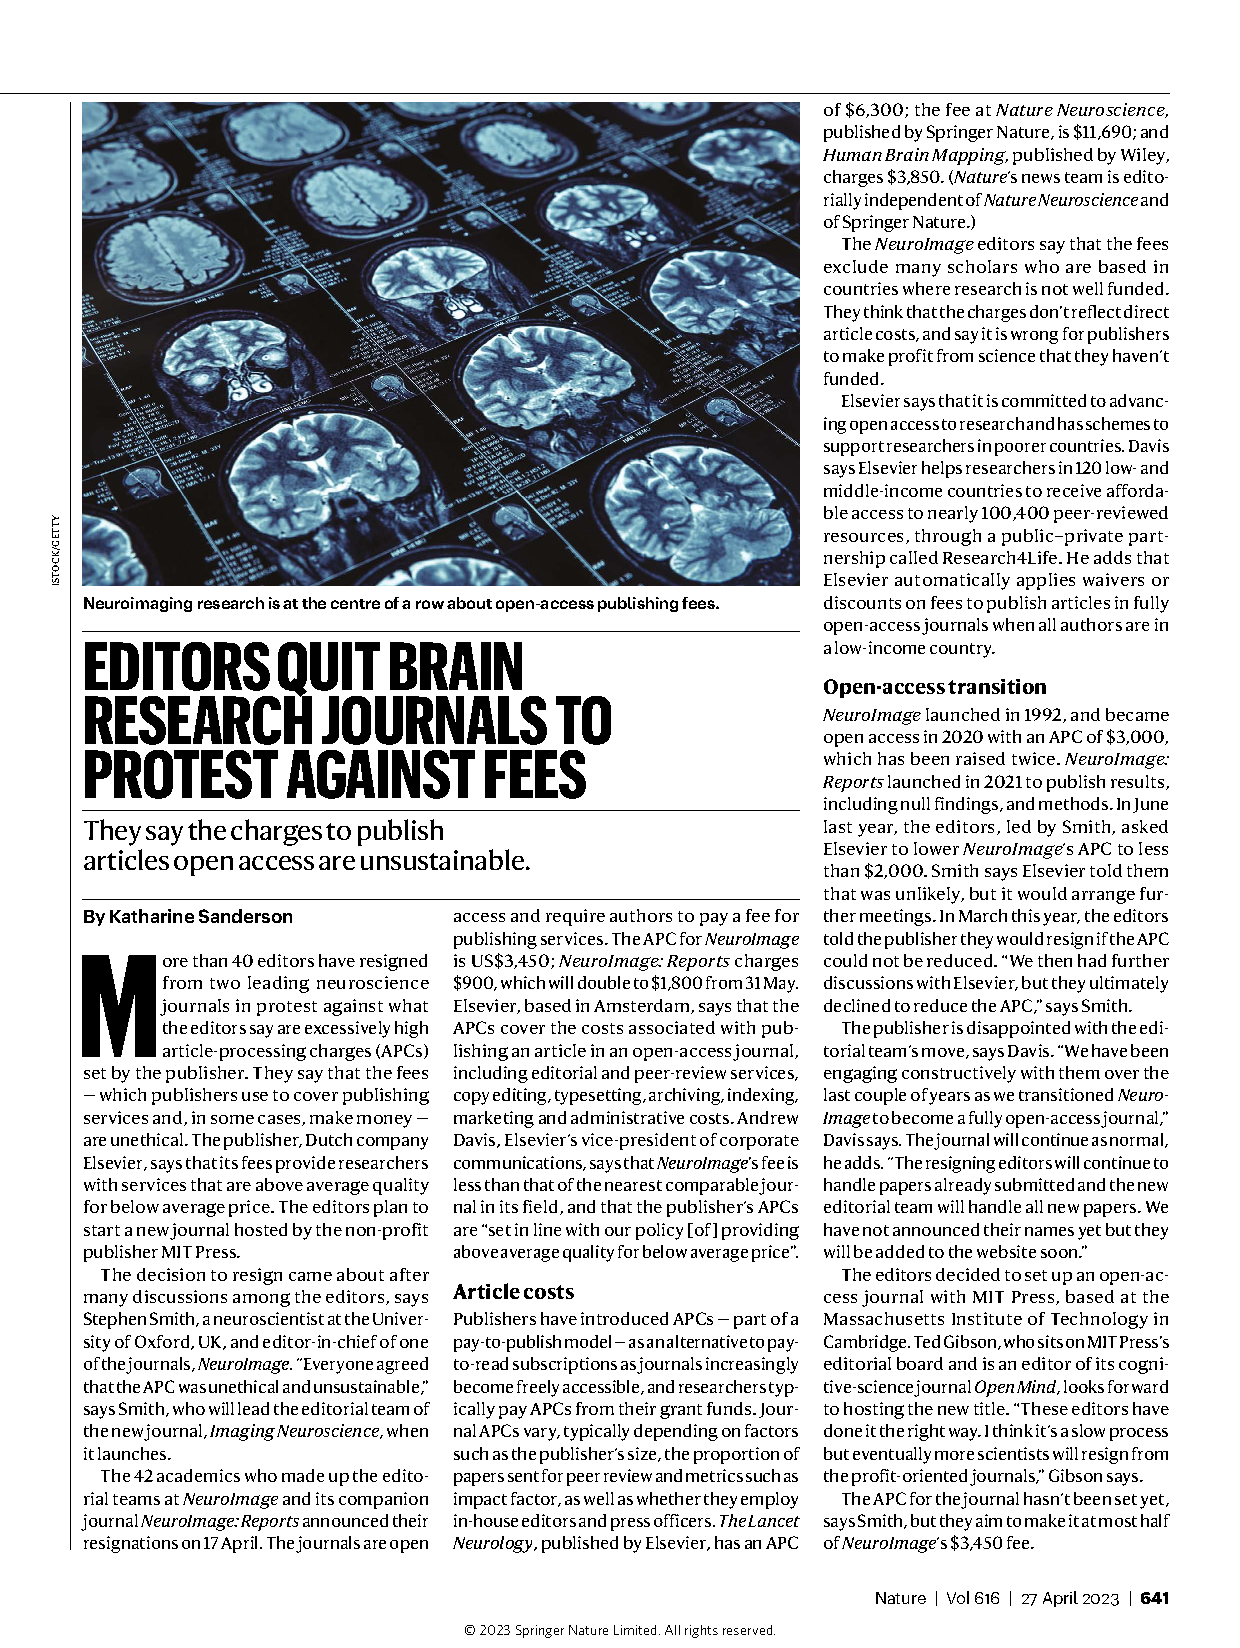
\includegraphics[width=.8\textwidth]{neuro-image-rebellion.pdf}
  \end{center}
\end{frame}

%%%

\subsection{APC agreements}
\begin{frame}[t]{Elsevier agreement}

\href{https://www.swissuniversities.ch/fr/themes/open-science/negociations-avec-les-editeurs/elsevier}{Negociations with Elsevier -- update 14th june 2024}
\begin{itemize}
  \item illimited access
  \item illimited open publications
  \item all journals
  \item All possible AI usage
  \item cost ?
\end{itemize}
\end{frame}



%%%

\section{Diamond Open Access}

 \begin{frame}[t]
  \begin{center}
  \vspace{3cm}
  {\huge The \textbf{Diamond Open Access} alternative}\\
  \end{center}
\end{frame}

%%%

\subsection{JTCAM presentation}
\begin{frame}[t]{}

\fig{.6}{logo2023}\newline

  \begin{quote}
    is a {\huge \textbf{Diamond open access}} journal, i.e. published with \textbf{no fees to either reader or author.} \newline
\end{quote}

  \begin{quote}
      and is an {\huge \textbf{overlay}} journal, i.e. that does not produce its own content, but selects from texts that are \textbf{already freely available online} (thanks to \href{https://www.episciences.org/}{Episciences!}).
\newline
\end{quote}

\pause

 \begin{itemize}
 \item Editorial process entirely controlled by researchers (Reviews, Copy-editing)
 \item Supported by \textit{Centre for Direct Scientific Communication} (CCSD@CNRS/INRAE/Inria)
 \item Wide spectrum: theoretical, applied, numerical, experimental
 \pause
 \item Publish \textbf{Open Reviews}
 \item Include \textbf{Dataset curation} (\textit{ETH-Board} support)
 \end{itemize}
\end{frame}

%%%

\subsection{Publication process}
\begin{frame}[t]{JTCAM: publication process}
 \begin{center}%
   \only<1>{\fig{1}{epirevue_0d}}%
   \only<2>{\fig{1}{epirevue_1d}}%
   \only<3>{\fig{1}{epirevue_2d}}%
    \only<4>{\fig{1}{epirevue_3d}}%
   \only<5>{\fig{1}{epirevue_4d}}%
   \only<6>{\fig{1}{epirevue_5d}}%
 \end{center}%
\end{frame}
 

%%%

% \subsection{Problematic of science metrics}
% \begin{frame}[t]{Problematic of bibliographic metrics}
% 
%   \begin{itemize}
%   \item Incentive to always \textbf{increase} the number of publications
%   \item Authors \textbf{fear} for their impact (for young investigators careers)
%   \item Journal \textbf{reputation} takes time to build
%   \item Imbalance between countries incentives (rich vs. poorer countries)
%   \end{itemize}
% 
%   \vfill
%   
%   \textbf{San Francisco Declaration on Research Assessment (DORA, 2013)}
%   \begin{quote}Do not use journal-based metrics, such as Journal Impact Factors, as a surrogate measure of the quality of individual research articles, to assess an individual scientist’s contributions, or in hiring, promotion, or funding decisions.\end{quote}
% 
%   \textbf{Coalition for Advancing Research Assessment (CoARA, 2022)}
% \begin{quote}
% The Agreement on Reforming Research Assessment sets a shared direction for changes in assessment practices for research, researchers and research performing organizations, with the overarching goal to maximize the quality and impact of research.
% \end{quote}
%   \vfill
%     
% \end{frame}
% %%%


\section{Open Data}
%%%

\subsection{What makes datasets useful ?}
\begin{frame}[t]{What makes (open) datasets useful: FAIR}

  \textbf{F}indable
  \begin{itemize}
    \item Searchable databases
    \item Annotation (keywords, cross-links, ownership, ...)
    \item \textit{Digital Object Identifier} (DOI)
  \end{itemize}
\vfill
  \textbf{A}ccessible
  \begin{itemize}
    \item Retention times?
    \item Data repository?
    \item Storage costs?   
  \end{itemize}
  \vfill
  \textbf{I}nteroperable
  \begin{itemize}
  \item Compatibility issues (between repositories, packages, file formats, ...)
  \end{itemize}
\vfill
  \textbf{R}eusable
  \begin{itemize}
    \item Operating context (Software versions, dependencies, ...)
    \item Open (source) licenses
  \end{itemize}

\end{frame}

%%%


\subsection{Journals policies with datasets}
\begin{frame}{Journals policies with datasets}


e.g. the \href{https://www.springernature.com/gp/authors/research-data-policy}{Springer research data policy}\newline

\href{https://group.springernature.com/gp/group/media/press-releases/archive-2016/over-600-springer-nature-journals-commit-to-new-data-sharing-policies/12000254}{Classification of journals}
\begin{tabular}{ll}
 Type 1 & Data sharing and data citation is encouraged                            \\
 Type 2 & Data sharing and evidence of data sharing encouraged                    \\
 Type 3 & Data sharing encouraged and statements of data availability required    \\
 Type 4 & Data sharing, evidence of data sharing and peer review of data required \\
\end{tabular}\newline\newline
\pause
$\Rightarrow$ \textbf{(Computational) mechanics should be of type 4}
\pause
\vfill

\begin{itemize}
  \item Springer journals created to review datasets (\href{https://www.springernature.com/gp/authors/research-data/research-data-publishing}{Scientific Data, BMC series, Discover})
  \item The \href{https://joss.theoj.org/about}{Journal of Open Source Software (JOSS)}, Open Source Initiative\\
\pause
  \item and now \href{https://jtcam.episciences.org/}{JTCAM} $\Rightarrow$ ambitious goals
\end{itemize}
\pause
\vfill
\begin{center}
{\Large Makes sense to gather the review of paper and datasets}
\end{center}
\begin{center}
\pause
    {\alert{\Large My personal belief is that journals should play a role}}
\end{center}

\end{frame}


%%%

\subsection{JTCAM dataset curation policy}
\begin{frame}{JTCAM dataset curation policy}

The following criteria are required in order to accept a submission to the JTCAM community:

\begin{itemize}
\item Must be Open Access
\item Ownership described in depth
\item Detailed description (using standard ontologies or controlled vocabularies)
\item Cross-linked reference must be added
\item Software permanent links (Software Heritage)
\item Acknowledged grants
\item Cleaned (no unnecessary files/folders or redundancy)
\item Permissive licenses are required (CC0, CC-BY-4.0)
\item Files formats are open
\item Workflow description
\end{itemize}

\vfill
  \url{https://zenodo.org/communities/jtcam/curation-policy}

\end{frame}

%%%

\subsection{Ideal curation tool}
\begin{frame}[t]{Ideal curation}
  \vspace{1.5cm}
    {\large
  \begin{itemize}
    \item \textbf{Versatile} data storage
    \item \textbf{Various} disciplines (experimental, theoretical, numerical, fluid mechanics, solid mechanics, ...)
    \item Collaborative curation (\textbf{concurrent editing})
    \item Robust descriptions (\textbf{ontologies})
    \item Reproducibility (\textbf{workflows})
\end{itemize}
}
\end{frame}


%%%


\section{DCSM and solidipes}
\subsection{DCSM project context}
\begin{frame}{DCSM Project}

Project \textbf{Dissemination of Computational Solid Mechanics}(DCSM)\\
\begin{itemize}
  \item Fund by \href{https://ethrat.ch/en/eth-domain/open-research-data/}{Open Research Data (ORD)}
  \item G. Anciaux (dev and supervision@EPFL), S. Pham-Ba (developer@EPFL)
  \item Young project (18 months)
  \item Use lots of project dependencies  
\end{itemize}
\vfill
\textbf{Goals}
\begin{itemize}
  \item Provide a \textbf{cloud based} repository/storage/tool for \textbf{solidmechanics} community
  \item Simplify the \textbf{verification, analysis and annotation} (curation) of datasets
  \item Stand-alone tool for researchers to manipulate data \textbf{on their personal computer}
  \item Web service: \url{https://dcsm.epfl.ch}
  \item Used at JTCAM for \textbf{data reviews}
  \item \textit{``Overleaf''} for datasets
\end{itemize}
\end{frame}
%%%

\subsection{Solidipes curation steps}
\begin{frame}{\fig{.025}{swiss-flag} Solidipes: analysis and curation tool}

\begin{enumerate}
  \item Access remote data-storage/repository (S3, ssh, Windows share)
\pause
  \item Scan files
\pause
  \item For each file
 \begin{itemize}
   \item Identify the encoding/file format
   \item Extract the metadata (CSV headers, image properties, finite element field descriptions)
   \item Attempt a (partial) loading of the file
   \item If any perform additional validation checks
 \end{itemize}
\pause
\item Generates a validating report in either
 \begin{itemize}
   \item text mode (terminal)
   \item Jupyter notebook
   \item WebApp allowing graphical scrutiny (images, interactive 3D rendering, ...)
\end{itemize}
\pause
\item If validated: enables export to Zenodo/Renku
 \end{enumerate}
\end{frame}


%%% 

\subsection{Solidipes examples}
\begin{frame}{\fig{.025}{swiss-flag} Solidipes: analysis and curation tool}

\begin{minipage}{.6\textwidth}
  \textbf{Features}
\begin{itemize}
  \item Analysis: Jupyterlabs and context preserving
  \item Curation: dedicated readers\&viewers (web oriented)
  \item Export/Import/Mount (S3, samba, nfs, Zenodo repositories)
  \item Operating Context saved (\textbf{Docker} containerization)
\end{itemize}
\vfill
\textbf{Demo}
\begin{itemize}
  \item {\footnotesize E. Eid, R. Seghir, \& J. Réthoré. Accompanying data for the paper "Crack branching at low tip speeds: spilling the T"}
\item \href{https://doi.org/10.5281/zenodo.8256346}{Zenodo}
\item \href{https://renkulab.io/projects/guillaume.anciaux/jtcam-data-10172}{@Renku} (\textit{a platform and tools for reproducible and collaborative data analysis})
\item \href{https://renkulab.io/projects/guillaume.anciaux/jtcam-data-10172/sessions/new?autostart=1}{Curation session}
\end{itemize}
\end{minipage}
\begin{minipage}{.39\textwidth}
\fig{.7}{solidipes-icon}
\end{minipage}
\end{frame}
%%%

\subsection{Solidipes philosophy}
\begin{frame}{\fig{.025}{swiss-flag} Solidipes: analysis and curation tool}
  \only<1>{\fig{.8}{dcsm_principle-9}}
  \only<2>{\fig{.8}{dcsm_principle-8}}
  \only<3>{\fig{.8}{dcsm_principle-7}}
  \only<4>{\fig{.8}{dcsm_principle-6}}
  \only<5>{\fig{.8}{dcsm_principle-5}}
  \only<6>{\fig{.8}{dcsm_principle-4}}
  \only<7>{\fig{.8}{dcsm_principle-3}}
  \only<8>{\fig{.8}{dcsm_principle-2}}
  \only<9>{\fig{.8}{dcsm_principle-1}}
\end{frame}
%%%

%\subsection{Data Curation process@JTCAM}
%\begin{frame}[t]{Dataset Curation Management@JTCAM}
%\fig{.8}{data_curation}
%\end{frame}
%
%%%

\subsection{Solidipes project (renewed version)}
\begin{frame}{Solidipes project}
\textbf{Solidipes: an interoperable tool for curation of research data}
  \begin{itemize}
  \item Fund by \href{https://ethrat.ch/en/eth-domain/open-research-data/}{Open Research Data (ORD)}
  \item G. Anciaux (LSMS), S. Pham-Ba (ENAC-IT4R), A. Borel (EPFL Library), V. Savchenko and
A. Neronov (LASTRO)
  \item 18 more months
\end{itemize}
\vfill
\textbf{Goals}
\begin{itemize}
 \item \textbf{Generalizing} Solidipes for virtually all fields
 \item \textbf{Extending} to view workflows
 \item \textbf{Integrating} with other storage repositories (import/export)
 \item \textbf{Integrating} with new services (Galaxy, MMODA)
 \item \textbf{Distribute} plugins contributed by distinct scientific communities.
\end{itemize}
\end{frame}
%%%

\begin{frame}{How to create a scientific field}
  \begin{minipage}{.56\textwidth}
\textbf{Solidipes components}\newline \newline
  \fig{.5}{solidipes-constituents}
\end{minipage}
  \begin{minipage}{.4\textwidth}
\textbf{Loader\&Viewers}
  \begin{itemize}
    \item image, notebook, text, pdf, code\_snippet, video, hdf5, python\_pickle, table, xml
    \item meshio, abaqus
 \end{itemize}

\vfill

\textbf{Validations}
  \begin{itemize}
    \item Mime type \textbf{matches} extension
    \item CSV \textbf{have} headers
    \item General: data \textbf{fall} into a category
  \end{itemize}

\end{minipage}
\end{frame}

%%%

\section{Ontologies}
\subsection{Ontology definition and description}
\begin{frame}[t]{Ontologies}

    \textbf{Ontology (adapted from Wikipedia)}
\begin{quote}
an ontology encompasses \textbf{definitions} of the \textbf{categories}, \textbf{properties}, and \textbf{relations} between the \textbf{data entities} of a \textbf{(scientific) topic}.
  \end{quote}
\pause
\vfill
\begin{minipage}{.4\textwidth}
In practice it is an \textbf{annotated graph} described with the \textit{Resource Description Framework}  (\href{https://www.techtarget.com/searchapparchitecture/definition/Resource-Description-Framework-RDF}{RDF})\newline
\pause
\vfill
e.g. a {\huge \textbf{valid}} mesh file {\huge\textbf{must}} contain nodes and elements. 
\end{minipage}
\begin{minipage}{.56\textwidth}
\begin{center}
  \fig{.55}{ontology-exemple}
\end{center}
\end{minipage}

\vfill
\pause
\begin{itemize}
  \item \href{https://www.xdmf.org/index.php/XDMF_Model_and_Format}{XDMF} is a XML file (detected by linux) containing \textit{nodes and elements} tags
  \item \textbf{.inp} is the \textbf{Abaqus} input file format, which may, or may not include meshing information
\pause
  \item \alert{Will allow semi-automatic validation, and content check for specific purpose}
\end{itemize}
\vfill
% Ontology repository: \url{schema.org}
  \end{frame}

%%%

% \subsection{Ontologies for Astronomy}
% \begin{frame}[t]{Ontologies in Astronomy}
%     
% The \href{https://www.ivoa.net/rdf/}{International Virtual Observatory Alliance (IVOA), 2002}
% \begin{quote}
%     is an organisation that debates and agrees the technical standards that are needed to make the VO possible. [...]
%   \end{quote}
% \begin{center}
%   \fig{1}{paper-astro}
% \end{center}
% \end{frame}

%%%


\subsection{Store ontologies and metadata}
\begin{frame}{Ontologies}
\textbf{ROcrate}
\begin{itemize}
  \item Adopt ``ro-crate-metadata.json''.
  \item \href{https://www.researchobject.org/ro-crate/specification/1.2-DRAFT/metadata}{ROcrate Metadata}
  \item \href{https://www.dublincore.org/specifications/dublin-core/dcmi-terms/}{Dublin Core standard}
  \item \href{https://www.rohub.org}{ROHub}
\end{itemize}
\vfill
\textbf{Ontology Viewers ?}
\begin{itemize}
  \item RDF: (xml or Turtle-ttl) 
  \item RDFLib (python library) 
  \item JSON-LD https://json-ld.org/ (Schema.org)
\end{itemize}
\end{frame}


%%% 


\subsection{Ontologies for Mechanics}
\begin{frame}[t]{Ontologies in mechanics}

\textbf{J.-L. Hippolyte, P. Duncan, M. Bevilacqua and M. Chrubasik}. \textit{Ontologies for Experimental Mechanics}. British Society for strain measurement, National Physical Laboratory, Hampton Rd, Teddington TW11 0LW, UK. 2022 [\href{https://www.bssm.org/media/smjj4h43/ontologies-for-experimental-mechanics.pdf}{link}]
\vfill
\textbf{Marcin Skulimowski}. \textit{An OWL Ontology for Quantum Mechanics}. Faculty of Physics and Applied Informatics, University of Lodz. Pomorska 149/153, 90-236 Lodz, Poland. 2002 [\href{https://ceur-ws.org/Vol-614/owled2010_submission_18.pdf}{link}]
\vfill

\textbf{H.A. Preisig, T.F. Hagelien, J.Friis, P. Klein, N. Konchakova}. \textit{Ontologies in Computational Engineering}. 14th World Congress on Computational Mechanics (WCCM). 2020. [\href{https://www.scipedia.com/wd/images/d/dd/Draft_Content_689054725p3366.pdf}{link}]

\vfill
\pause
\begin{center}
\Large
  \alert{Need to integrate and mix these initiatives: Forming a committee ?}
\end{center}
\end{frame}


%%%

\section{Reproducibility}
\subsection{workflow}
\begin{frame}[t]{Reproducibility with workflows}
  \only<1>{\fig{.9}{simulation-flow-1.pdf}}
  \only<2>{\fig{.9}{simulation-flow-2.pdf}}
  \only<3>{\fig{.9}{simulation-flow-3.pdf}}
  \only<4>{\fig{.9}{simulation-flow.pdf}}
  \only<5->{\vspace{-1cm}
 \fig{.6}{simulation-flow-pkg.pdf}}
\only<6>{
\begin{minipage}{.5\textwidth}
\begin{itemize}
  \item \textbf{Docker} container: \href{https://renkulab.io/}{Renku}, \href{https://mybinder.org/}{Binder}, ...
  \item \textbf{Worflow} management: \href{https://www.aiida.net/}{AiiDA}, \href{https://blackdynamite.readthedocs.io/en/latest/}{BlackDynamite}
  \item \textbf{Packagers}: \href{https://www.researchobject.org/ro-crate/}{ROcrate}, \href{https://www.reprozip.org/}{reprozip}
  \item \textbf{Repository}: \href{https://workflowhub.eu/}{WorkflowHub} 
  \end{itemize}
\end{minipage}
\begin{minipage}{.45\textwidth}
\textbf{Acquiring OS context \newline + ``automatic'' DockerFiles?}
\end{minipage}
}
\end{frame}

%%%
\section{Conclusion}
\subsection{publishing system}
\begin{frame}[t]{Conclusion (open access)}

  \textbf{Open access problematic}  
  \begin{itemize}
  \item Public money must turn into public knowledge and goods
  \item Edition has intrinsic costs, but unreasonable APCs are not acceptable
  \item Current system leads to explosion of publications and costs
  \end{itemize}
\vfill
  \textbf{Diamond Open access alternatives}  
  \begin{itemize}
  \item No fees to authors nor reader => \textbf{public good}
  \item Freedom for researchers: \textbf{ethics} and \textbf{quality} can be the driving force
  \item Needs support from institutions (see \href{https://www.swissuniversities.ch/en/topics/open-science/open-science-programme/chord}{SwissUniversities} and \href{https://ethrat.ch/en/measure-1-calls-for-field-specific-actions/}{ETH-Board ORD} programs
  \item \href{https://www.unesco.org/en/articles/announcing-global-diamond-open-access-alliance}{UNESCO Diamond Open Access Global Alliance} is born
  \item Unclear link with bibliographic metrics
  \item \textbf{JTCAM}: a healthy Diamond open access journal, with innovative dataset handling
  \end{itemize}
\vfill
\begin{center}
\Large  \textbf{Researchers can be game changers, if they want to...}
\end{center}
\end{frame}

%%%


\begin{frame}[t]{Conclusion (data curation)}

  \textbf{Where is Solidipes}  
  \begin{itemize}
  \item \textbf{Data curation} with loaders/viewers (mostly for continuum solidmechanics)
    \pause
  \item \textbf{Flexible} (remote) data storage
    \pause
  \item Publication and archive on \textbf{Zenodo/Renku + {\color{red} dtool}}
    \pause
  \item \textbf{JTCAM curation policy} enforced with Solidipes@DCSM already\\\pause
  $\Rightarrow$ Brings good principles to this Diamond open access initiative
  \item User \textbf{Documentation}
  \end{itemize}
  \pause
  \vfill
  \textbf{Next steps}
  \begin{itemize}
    \item Ontologies $\Rightarrow$ \textbf{Automatic and Robust} validation\&recognition (reviewer friendly)
    \item Complete workflow remains a \textbf{manual} task $\Rightarrow$ guaranty reproducibility
    \item \textbf{Plugins} remain to be contributed ({\color{red} contact us})
  \end{itemize}
\vfill
\end{frame}
%%% 


\begin{frame}[t]{You are a Research Software Engineer}
\large
  \begin{itemize}
\item You have a job in research? You write software? → \textbf{You are an RSE!}
\item We often lack recognition/career progression despite contributions\newline 
\vfill
→ \textbf{Join RSE communities !}
\vfill
\item Associations at international, national, instutitional scale
\url{https://researchsoftware.org/assoc.html}
\item Networking and events (\href{https://rsecon24.society-rse.org/}{RSE CON 24})
\item Acquire skills for managing projects and building careers
\end{itemize}
\end{frame}

%%%


\end{document}
